\documentclass{article}
\usepackage[T1]{fontenc}

\usepackage{graphicx}
\usepackage{listings}
\begin{document}

\title{FOSS Lab Report}
\author{Gokul K\\[2\baselineskip]
Roll Number: 21\\[2\baselineskip]}
\date{25 January 2020}

\maketitle

\setcounter{section}{6}
\section{Shell Programming IV}
\subsection{Aim}
Write a script called addnames that is to be called as follows ./addnames ulist username
Here ulist is the name of the file that contains list of user names and username is a
particular student’s username. The script should
   i) check that the correct number of arguments was received and print a message, in
    case the number of arguments is incorrect
   ii) check whether the ulist file exists and print an error message if it does not
   iii) check whether the username already exists in the file. If the username exists, print a message stating that the name already exists. Otherwise, add the username to the end of the list

\subsection{Source Code}
\begin{verbatim}
#! /bin/bash

if [[ $# -ne 2 ]]
then
	echo "Invalid number of arguments"
	exit
fi

if [[ ! (-a $1) ]]
	then
	echo "Not a valid file location or file dosent exist"
	exit
fi

NO=$(grep -c -e $2 $1)
if [[ $NO -eq 0 ]]
then
	echo $2 >> $1
	echo "Username is added"
	exit

else
	echo "Username already exists"
	exit
fi
\end{verbatim}

\subsection{Output}
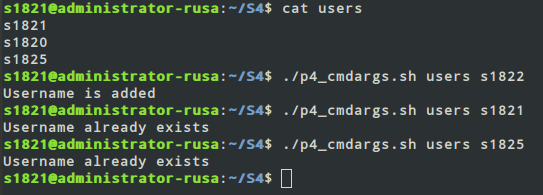
\includegraphics[width=0.9\textwidth]{img/p7/ss.png}\newline

\subsection{Result}
The above program is run on the server shell. Inputs which is both present in the users_list file and not present where given and corresponding outputs where recorded.
\end{document}